\section{Theorie}\label{sec:theorie}

\subsection{Kristallgitter}\label{subsec:kristallgitter}
Um das Material \heo, sowie die Röntgendiffraktometrie verstehen zu können, ist ein grundlegendes Verständnis
über die Struktur kristalliner Festkörpern unerlässlich.
Die nachfolgenden Seiten dienen also als Zusammenfassung für die relevanten Konzepte der Festkörperphysik.

\subsubsection{Bravaisgitter, Elementarzelle und Basis}
Als Idealisierung vieler Festkörper wird als Modell des idealen Kristalls herangezogen.
Ein idealer Kristall ist eine dreidimensionale, unendlich ausgedehnte Anordnung, die sich aus identischen, periodisch
wiederkehrenden Baueinheiten zusammensetzt.
Diese Baueinheiten werden als Basis bezeichnet.
Sie können einzelne Atome, aber auch komplexe Atomstrukturen repräsentieren.
Reduziert man jede Baueinheit auf einen einzigen Punkt, so entsteht ein einfach zu beschreibendes Punktgitter.
\autocite[49]{Hunklinger}
Dieses unterliegt verschiedenen Symmetrien, sodass das Gitter in unterschiedliche Kristallsysteme eingeteilt werden
kann.
Eine einfache Einteilung kann mithilfe von Drehachsen erfolgen.
Hierbei betrachtet man diejenigen Rotationsoperatoren $R_{\hat{e}}(2\pi / n)$ für eine beliebige Achse $\hat{e}$ um
einen Winkel $2 \pi /n$, die das Punktgitter auf sich selbst abbilden.
Der Parameter $n$ wird als Zähligkeit bezeichnet und teilt die Punktgitter in sieben verschiedene Kristallklassen ein,
die in Tabelle \cref{tab:krystallsysteme} aufgeführt sind.
\autocite[53]{Hunklinger}
\begin{table}[h]
    \centering
    \begin{tabular}{c c c c}
        \toprule
        Kristallsystem           & Gitterkonstanten  & Winkel                                       & Zähligkeit \\ \midrule
        triklin                  & $a \neq b \neq c$ & $\alpha \neq\beta \neq\gamma$                & 1          \\
        monoklin                 & $a \neq b \neq c$ & $\alpha=\gamma=\ang{90},\beta \neq \ang{90}$ & 2          \\
        orthorhombisch           & $a \neq b \neq c$ & $\alpha=\beta=\gamma=\ang{90}$               & 2 (zwei)   \\
        tetragonal               & $a = b \neq c$    & $\alpha=\beta=\gamma=\ang{90}$               & 4          \\
        hexagonal                & $a = b \neq c$    & $\alpha=\beta=\ang{90}, \gamma=\ang{120}$    & 6          \\
        trigonal (rhomboedrisch) & $a=b=c$           & $\alpha=\beta=\gamma \neq \ang{90}$          & 3          \\
        kubisch                  & $a=b=c$           & $\alpha=\beta=\gamma=\ang{90}$               & 3 (vier)   \\ \bottomrule
    \end{tabular}
    \caption{Klassifikation der verschiedenen Kristallsysteme. \imcite[65]{Hunklinger} }\label
    {tab:krystallsysteme}
\end{table}


Eine weitere wichtige Symmetrie ist die Translationssymmetrie.
Betrachtet man diejenigen Translationsoperatoren $T(\mathbf{O})$, die das Gitter auf sich selbst abbilden, dann erkennt
man aufgrund der Periodizität des Gitters den Zusammenhang
$\mathbf{O} = n_{1}\mathbf{a}_{1}+n_{2}\mathbf{a}_{2}+n_{3}\mathbf{a}_{3}$, wobei
$\mathbf{a}_{i}\in\mathbb{R}^{3}, n_{i}\in\mathbb{Z}$. \autocite[50]{Hunklinger}
Die Vektoren $\mathbf{a}_{i}$
definieren ein schiefwinkliges Koordinatensystem und werden als primitive Gittervektoren bezeichnet.
Sie spannen ein dreidimensionales Bravaisgitter auf.
Die Abstände zwischen zwei benachbarten Gitterpunkten, also die Größen
$\lvert \mathbf{a}_{i} \rvert$, werden Gitterkonstanten genannt. \autocite[82]{Ashcroft}
Je nachdem, wie sich das Kristallsystem unter Symmetrieoperationen verhält, ergeben sich unterschiedliche Bedingungen für
Gitterkonstanten und die Winkel zwischen den Gittervektoren.
Mithilfe der Definition einer Basis und eines Bravaisgitters lässt sich jeder ideale Kristall beschreiben.
Eine Kristallstruktur wird durch identische Kopien der Basis an jedem Punkt des Bravaisgitters aufgebaut.
\autocite[94-95]{Ashcroft}
Man kann Teilmengen des Ortsraumes geschickt wählen, die durch Aneinanderreihung den gesamten Raum lückenlos und
überlappungsfrei überdecken.
Solche Mengen nennt man Elementarzellen.
Wählt man die Elementarzelle so, dass sie nur einen Gitterpunkt enthält, tritt der Spezialfall einer primitiven
Elementarzelle ein.
Mit einer primitiven Elementarzelle lässt sich der Raum lückenlos und überlappungsfrei überdecken, indem man die Zelle
entlang der primitiven Gittervektoren verschiebt.
Eine einfache Konstruktion liefert ein Parallelepiped, welches von den drei Basisvektoren aufgespannt wird.
Das Volumen $V_\mathrm{EZ}= \lvert \mathbf{a}_1 \cdot (\mathbf{a}_2 \times  \mathbf{a}_3) \rvert$ dieses
Parallelepipeds, gibt das effektive Volumen pro Gitterpunkt an.
\autocite[90-91]{Ashcroft}


Da man die Symmetriebeziehungen voll ausschöpfen möchte, benutzt man meist keine primitiven Elementarzellen, sondern
wählt geschickt nicht-primitive Elementarzellen, die möglichst viele Punktsymmetrieelemente beinhalten.
Das führt zu einer Einteilung in 14 Bravaisgitter. \autocite[51]{Hunklinger}

\subsubsection{Relevante Gittertypen}
\begin{figure}
    \centering
    \begin{subfigure}[t]{0.3\textwidth}
        \centering
        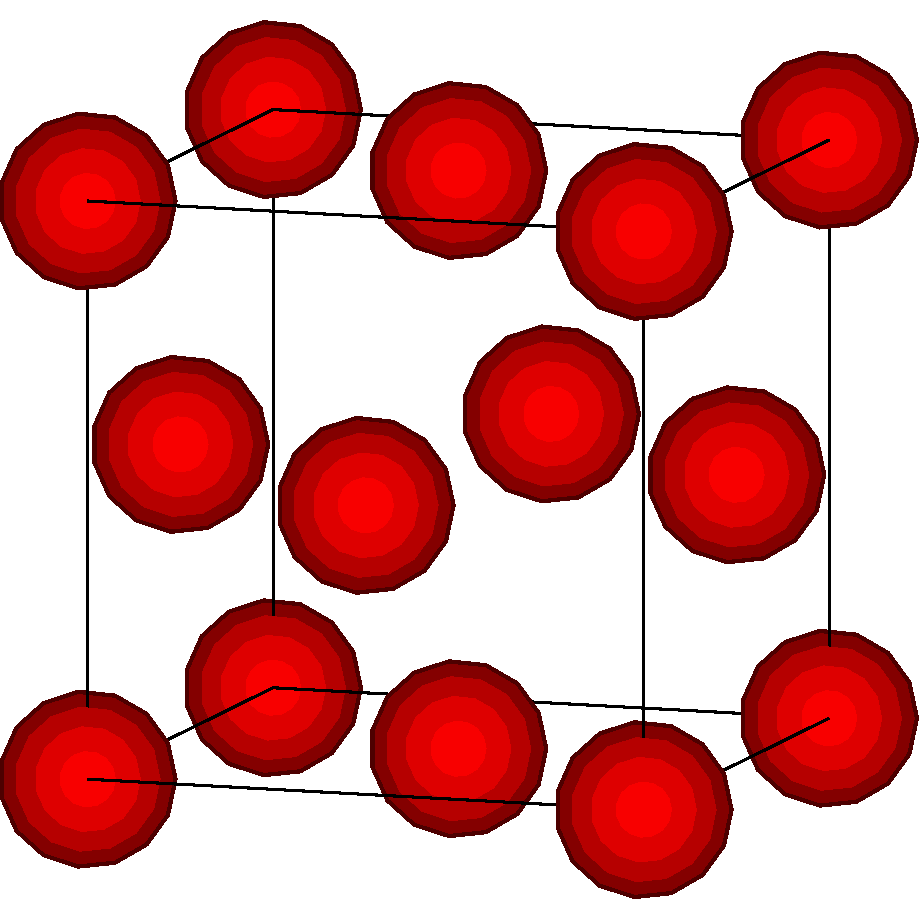
\includegraphics[width=\textwidth]{../assets/theorie/fcc}
        \caption{fcc-Gitter.} \label{fcc}
    \end{subfigure}
    \begin{subfigure}[t]{0.3\textwidth}
        \centering
        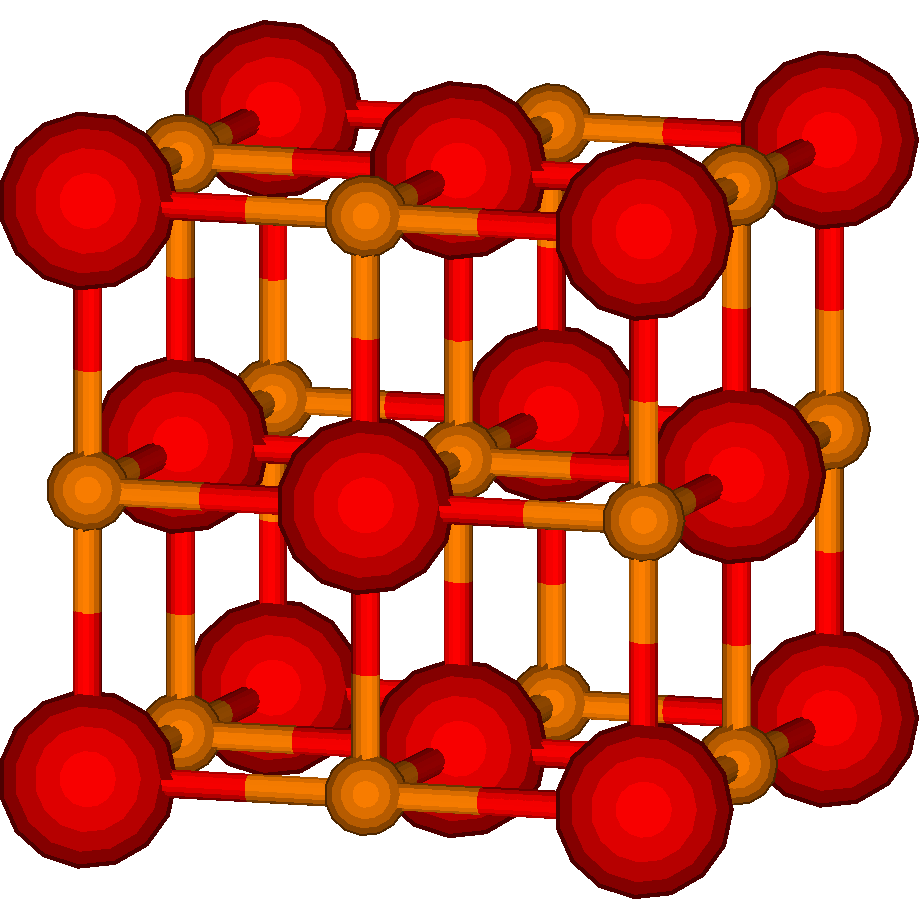
\includegraphics[width=\textwidth]{../assets/theorie/rocksalt}
        \caption{NaCl-Gitter} \label{nacl}
    \end{subfigure}
    \begin{subfigure}[t]{0.3\textwidth}
        \centering
        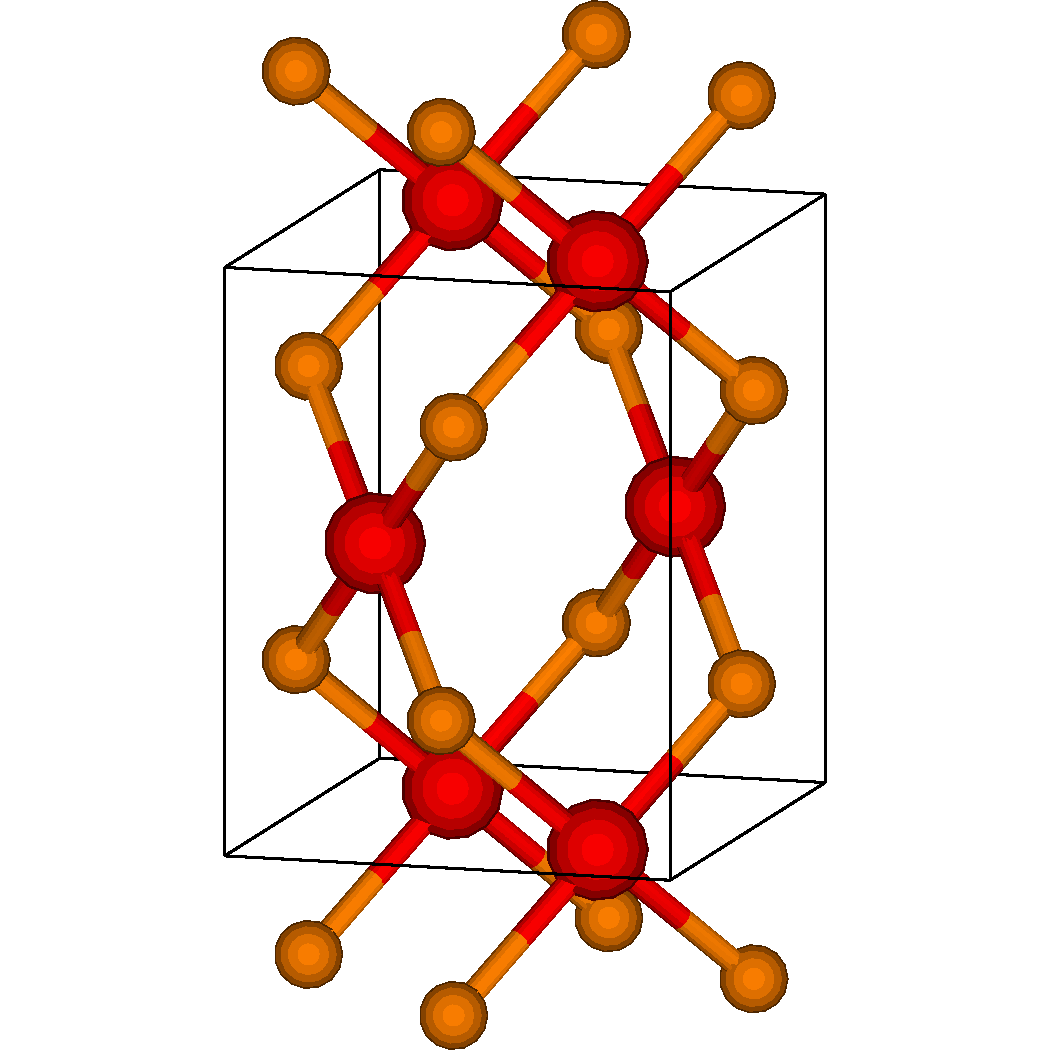
\includegraphics[width=\textwidth]{../assets/theorie/CuO}
        \caption{\ce{CuO}-Gitter} \label{cuo}
    \end{subfigure}
    \begin{subfigure}[t]{0.3\textwidth}
        \centering
        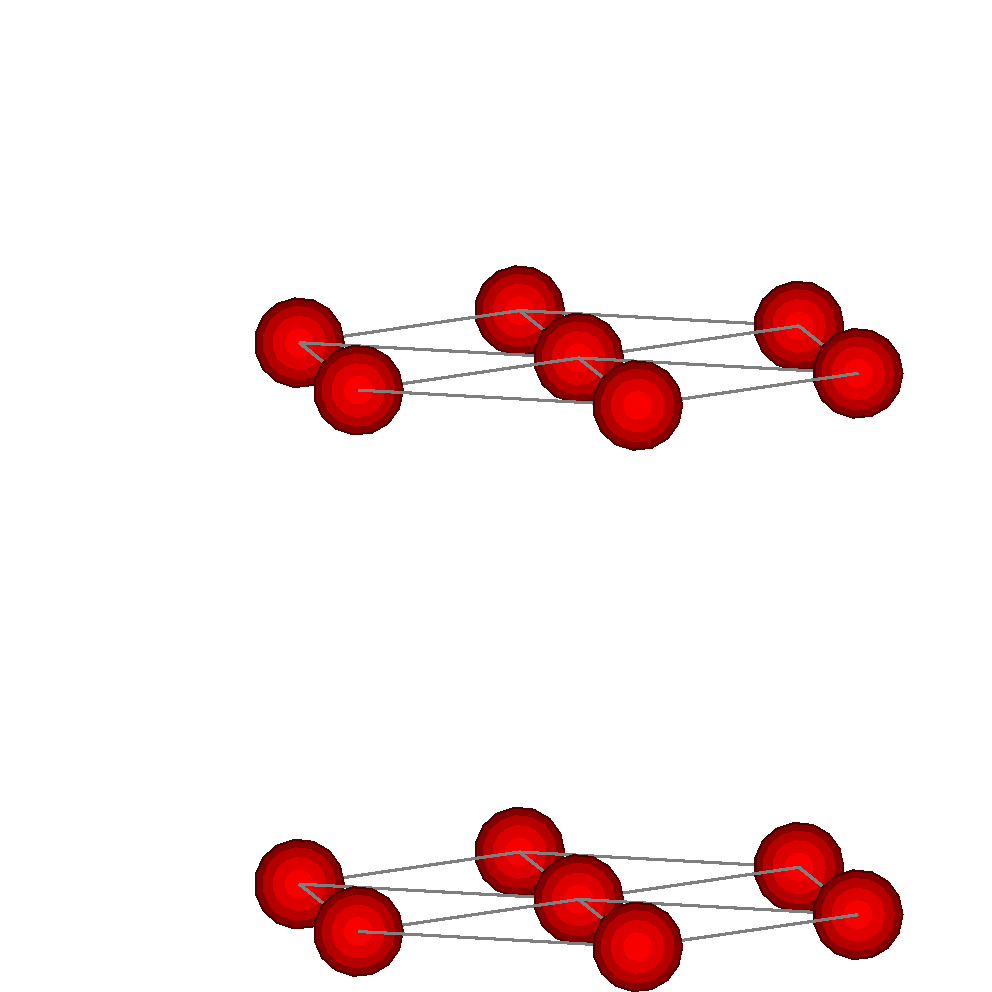
\includegraphics[width=\textwidth]{../assets/theorie/hex}
        \caption{hexagonales Gitter} \label{hex}
    \end{subfigure}
    \begin{subfigure}[t]{0.3\textwidth}
        \centering
        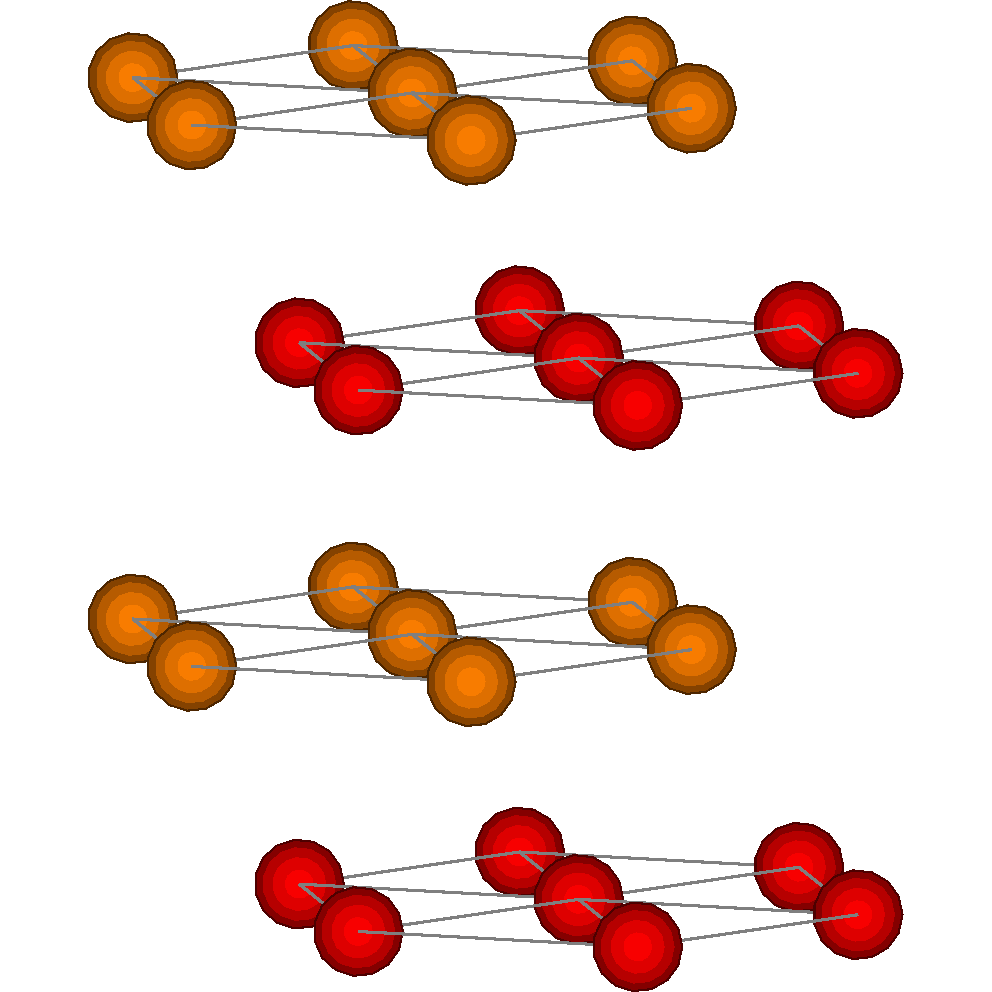
\includegraphics[width=\textwidth]{../assets/theorie/hcp}
        \caption{hcp-Gitter} \label{hcp}
    \end{subfigure}
    \begin{subfigure}[t]{0.3\textwidth}
        \centering
        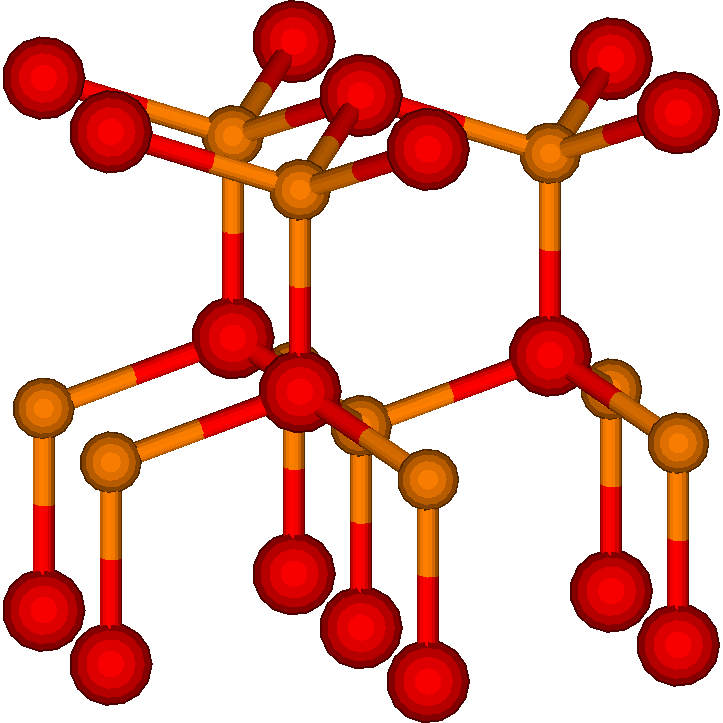
\includegraphics[width=\textwidth]{../assets/theorie/wurzite}
        \caption{Wurtzit-Gitter} \label{wurtzit}
    \end{subfigure}
    \caption{Relevante Gitterstrukturen für die Untersuchung von \heo.} \label{fig:gitterstrukturen}
\end{figure}

\paragraph{Natriumchloridstruktur}
Die erste und wichtigste Kristallstruktur ist die Natriumchloridstruktur.
Um diese zu verstehen, betrachtet man zuerst ein kubisch-flächen\-zen\-trier\-tes Gitter (fcc, engl.
\textit{face-centered cubic}) welches durch die primitiven Vektoren
\begin{equation*}
    \mathbf{a}_1 = a / 2 (\hat{x} + \hat{y}), \quad
    \mathbf{a}_2 = a / 2 (\hat{y} + \hat{z}), \quad
    \mathbf{a}_3 = a / 2 (\hat{x} + \hat{z})
\end{equation*}
definiert ist.
Die Gitterpunkte liegen an Würfelecken und den dazugehörigen Flächenmittelpunkten, wie in \cref{fcc} dargestellt.
\autocite[37-38]{Grundmann}
Die Natriumchloridstruktur entsteht aus einem fcc-Gitter mit zweiatomiger Basis.
Dabei ist das erste Basisatom an der Gitterposition $(0,0,0)$ und das zweite an der Position $(a/2,a/2,a/2)$, wie in
\cref{nacl} dargestellt.\autocite[45]{Grundmann}
Sowohl Magnesiumoxid \ce{MgO}, Kobaltoxid \ce{CoO} und Nickeloxid \ce{NiO} kristallisieren in dieser Struktur.
Das zu untersuchende hochentropische Metalloxid \heo\ soll ebenfalls in dieser Struktur kristallisieren, wenn
Sauerstoff als erstes Basisatom und ein zufällig ausgewähltes Metall als zweites Basisatom betrachtet wird.

\paragraph{Kupferoxidstruktur}
Kupferoxid kristallisiert in einer monoklinen Kristall\-struk\-tur mit achtatomiger Basis.
Dabei sind vier dieser Basisatome Kupferatome und vier Sauerstoffatome.
Die Struktur ist in \cref{cuo} dargestellt.\autocite[7]{kupferoxid}

\paragraph{Wurtzitstruktur}
Um die Wurtzitstruktur zu verstehen, betrachtet man zuerst die einfach-hexagonale Struktur, die durch die primitiven
Vektoren
\begin{equation*}
    \mathbf{a}_1 = a\hat{x}, \quad
    \mathbf{a}_2 = a/2 (\hat{x} + \sqrt{3} \hat{y}), \quad
    \mathbf{a}_3 = c \hat{z}
\end{equation*}
definiert ist.
Es entsteht ein Gitter, welches an den Ecken eines Sechsecks und den dazugehörigen Flächenmittelpunkten Gitterpunkte
besitzt, wie in \cref{hex} dargestellt.
Aus der einfach-hexagonalen Struktur ergibt sich die hexagonal dichtest gepackte Struktur
(hcp, engl. \textit{hexagonal-closed packet}).
Diese liegt ein einfach-hexagonales Gitter mit zweiatomiger Basis bei den Gitterpositionen $(0,0,0)$ und
$(\mathbf{a}_1/3 + \mathbf{a}_2/3 + \mathbf{a}_3/2)$ zugrunde, wie in \cref{hcp} dargestellt.\autocite[97-98]{Ashcroft}
Die Wurtzitstruktur besteht aus einem einfach-hexagonalen Gitter mit vieratomiger Basis.
Eine bessere Vorstellung ergibt sich jedoch aus der Betrachtung zweier übereinander liegender hcp-Gitter, die um
die Höhe $\sqrt {3 / 8} a$ gegeneinander verschoben sind, wie in \cref{wurtzit} dargestellt.
Zinkoxid \ce{ZnO} kristallisiert in dieser Struktur.

\subsubsection{Reziprokes Gitter}
Das reziproke Gitter spielt für die weitere Betrachtung von periodischen Strukturen eine fundamentale Rolle.
Ziel ist es, eine Funktion zu konstruieren, die gitterperiodisch im Bravaisgitter ist.
Für diese Funktion soll also gelten
$f(\mathbf{x})=f(\mathbf{x}+\mathbf{O})$, falls $\mathbf{O}=\sum_{i=1}^{3} \alpha_{i}\mathbf{a}_{i}$.
Mithilfe einer Reihenentwicklung erhalten wir die folgende, allgemeine Form:
\begin{align*}
    f(\mathbf{x})&=\sum_{\mathbf{R}}a_{\mathbf{R}}\cdot \exp(\mathrm{i}\mathbf{R}\cdot\mathbf{x}) \\
    f(\mathbf{x}+\mathbf{O})&=\sum_{\mathbf{R}}a_{\mathbf{R}}\cdot \exp(\mathrm{i}\mathbf{R}\cdot \mathbf{x})\cdot
    \underbrace{ \exp(\mathrm{i}\mathbf{R}\cdot \mathbf{O}) }_{ \stackrel{!}{=}1 }  \stackrel{!}{=} f(\mathbf{x})
\end{align*}
Erkennbar ist die notwendige Bedingung $\exp(\mathrm{i}\mathbf{R}\cdot \mathbf{O})=1$.
Dies ist äquivalent zur Aussage $\mathbf{R}\cdot \mathbf{O}=2\pi n$ mit $n \in \mathbb{N}_{0}$.
Damit lässt sich das reziproke Gitter durch die Menge
$\{ \mathbf{R} \,\vert\, \exp(\mathrm{i}\mathbf{R}\cdot \mathbf{O})=1 \quad
\forall \mathbf{O} \in \text{span}(\mathbf{a}_{i}) \}$ definieren. \autocite[108]{Ashcroft}
Analog zum Ortsraum lassen sich auch hier primitiven Vektoren mit folgender Vorschrift bilden:
\begin{align*}
    \mathbf{b}_{1} = 2\pi \cdot \frac{\mathbf{a}_{2} \times \mathbf{a}_{3}}{V_{\mathrm{EZ}}} \quad
    \mathbf{b}_{2} = 2\pi \cdot \frac{\mathbf{a}_{3} \times \mathbf{a}_{1}}{V_{\mathrm{EZ}}} \quad
    \mathbf{b}_{3} = 2\pi \cdot \frac{\mathbf{a}_{1} \times \mathbf{a}_{2}}{V_{\mathrm{EZ}}}
\end{align*}
Jeder Punkt im reziproken Gitter kann durch $\sum_{i=1}^{3} \beta_{i}\mathbf{b}_{i}$ mit $\beta_i \in \mathbb{Z}
$ beschrieben werden.
Es gelten die Relation $\mathbf{b}_{i}\cdot \mathbf{a}_{j}=2 \pi \delta_{ij}$.
Hierbei ist $\delta_{ij}$ das Kronecker-Delta.
\autocite[109]{Ashcroft}

\subsubsection{Indizierung von Gitterebenen und Gitterrichtungen}
Die erste wichtige Anwendung des reziproken Gitters ist die Charakterisierung von Gitterebenen.
Eine Gitterebene ist eine beliebige, im Bravaisgitter liegende Ebene, die mindestens drei nicht kollineare Gitterpunkte
enthält.
Aufgrund der Kristallsymmetrie liegen damit unendlich viele weitere Gitterpunkte innerhalb dieser Ebene.
Mithilfe der Translationssymmetrie findet man parallele Gitterebenen im Abstand $d$.
Diese fasst man als Gitterebenenscharen zusammen.

Nun kann man Gitterebenenscharen mithilfe des reziproken Gitters charakterisieren, denn für jede
Gitterebenenschar im Abstand $d$ existieren Vektoren des reziproken Gitters, welche senkrecht auf den Ebenen stehen.
Für die eindeutige Beschreibung wählt man den kleinsten dieser Vektoren, stets welche die Länge $2 \pi / d$ besitzt.
Auch die Umkehrung gilt: Für jeden Vektor $\mathbf{R}$ aus dem reziproken Gitter, existiert eine Schar von senkrechten
Gitterebenen.
Der Abstand $d$ dieser Ebenen ist an den Betrag den kleinsten parallelen Vektor $\mathbf{r}$ durch $\lvert \mathbf{r}
\rvert=2\pi  /d$ gekoppelt.
Es existiert also eine einfache Möglichkeit, Gitterebenen mithilfe von reziproken Gittervektoren eindeutig zu
identifizieren. \autocite[113]{Ashcroft}

Nun können die sogenannten Millerschen Indizes verwendet werden, um Gitterebenenscharen eindeutig zu bestimmen.
Sei dazu $\mathbf{r}$ der kürzeste reziproke Gittervektor, welcher senkrecht auf der zu charakterisierenden Ebene steht.
Dieser lässt sich darstellen durch $ \mathbf{r} = h \mathbf{b_1} + k \mathbf{b_2} + l \mathbf{b_3}$.
Das Tupel $(h\, k\,l)$ sind die Millerschen Indizes, welche definitionsgemäß aus ganzen Zahlen bestehen müssen.


Für die Millerschen Indizes existiert eine geometrische Interpretation, die es erlaubt, die Indizes im Ortsraum zu
visualisieren.
Für jede Gitterebene findet man ein entsprechendes $A$, sodass die Ebenengleichung $\mathbf{r} \cdot \mathbf{x} = A$
erfüllt ist.
Nun definieren wir die Durchstoßpunkte zwischen den durch die primitiven Vektoren $\mathbf{a}_i$ aufgespannten
Koordinatenachsen und der Ebene durch die Zahlen $x_{1}\mathbf{a}_{1}, x_{2}\mathbf{a}_{2}, x_{3}\mathbf{a}_{3}$.
Da die Durchstoßpunkte in der Ebene liegen, ist die Ebenengleichung $\mathbf{K}\cdot(x_{i}\mathbf{a}_{i})=A$ erfüllt und
man findet mit $\mathbf{K}\cdot\mathbf{a}_{1}=2\pi h$, $\mathbf{K}\cdot \mathbf{a}_{2}=2\pi k$,
$ \mathbf{K}\cdot \mathbf{a}_{3}=2\pi l$ folgenden Zusammenhang:
\begin{equation*}
    x_{1}=\frac{A}{2\pi h}, \quad x_{2}=\frac{A}{2\pi k}, \quad x_{3} =\frac{A}{2\pi l}
\end{equation*}
Kennt man die Achsendurchstoßpunkte $x_i$, kann man die Millerschen Indizes finden, indem man den Parameter $A$
kleinstmöglich wählt, sodass $h$, $k$ und $l$ ganzzahlig sind. \autocite[115]{Ashcroft}

Nicht nur Gitterebenen, sondern auch Gitterrichtungen lassen sich in ähnlicher Weise indizieren.
Das Tupel $[h\,k\,l]$ beschreibt diejenige Richtung, die durch den Vektor $\mathbf{O} = h\mathbf{a}_{1}+k\mathbf{a}_{2}+
l\mathbf{a}_{3}$ dargestellt werden.
Zu beachten ist, dass Richtungsvektoren in unserem Kontext im Ortsraum leben,
währenddessen Ebenennormalenvektoren durch Vektoren im reziproken Raum dargestellt werden.
Um dies zu verdeutlichen werden eckige anstelle der runden Klammern verwendet.
Es existiert weiterhin eine besondere Notation zur Kennzeichnung äquivalenter Gitterebenenscharen und Raumrichtungen.
In diesem Kontext bedeutet das, dass die Möglichkeit besteht, äquivalente Gitterebenenscharen und Raumrichtung durch
Symmetrieoperationen ineinander zu überführen.
Äquivalente Ebenen notiert man mit $\{h \,k\, l \}$, für Richtungen gilt entsprechend $\langle h\, k \, l \rangle$.
\autocite[116]{Ashcroft}

\subsubsection{Röntgenbeugung und die Laue Bedingung}
Ziel ist es, mithilfe von elektromagnetischer Strahlung und den bisherigen Überlegungen, Aussagen über die
Kristallstruktur eines Festkörpers zu gewinnen.
Genauer gesagt sucht man einen Formalismus, um die elastische Streuung am Kristallgitter zu beschreiben.
Für eine geeignete Wellenlänge der Photonen betrachtet man die typische zwischenatomare Entfernung von circa
\qty{1}{\angstrom}.
Aus der Optik ist bekannt, dass mindestens eine Wellenlänge gleicher Größenordnung genutzt werden
muss, um beide Punkte hinreichend genau aufzulösen.
Entsprechend muss die Photonenenergie in der Ordnung von
$\hbar \omega=hc / \lambda \simeq \qty{12.3}{\electronvolt}$ liegen.
Hierbei ist $\omega$ die Kreisfrequenz, $\lambda$ die Wellenlänge, $h$ das Plancksche Wirkungsquantum und $c$ die
Lichtgeschwindigkeit.
Solche Energien sind charakteristisch für Röntgenstrahlung.

Laue und Bragg entwickelten zwei Formalismen, um die Physik hinter der Gitterstreuung zu verstehen.
Im Folgenden wird der Laue-Formalismus erklärt und die Äquivalenz zur Bragg-Bedingung gezeigt.

\paragraph{Beugungsbedingung nach Laue}
\begin{figure}
    \centering
    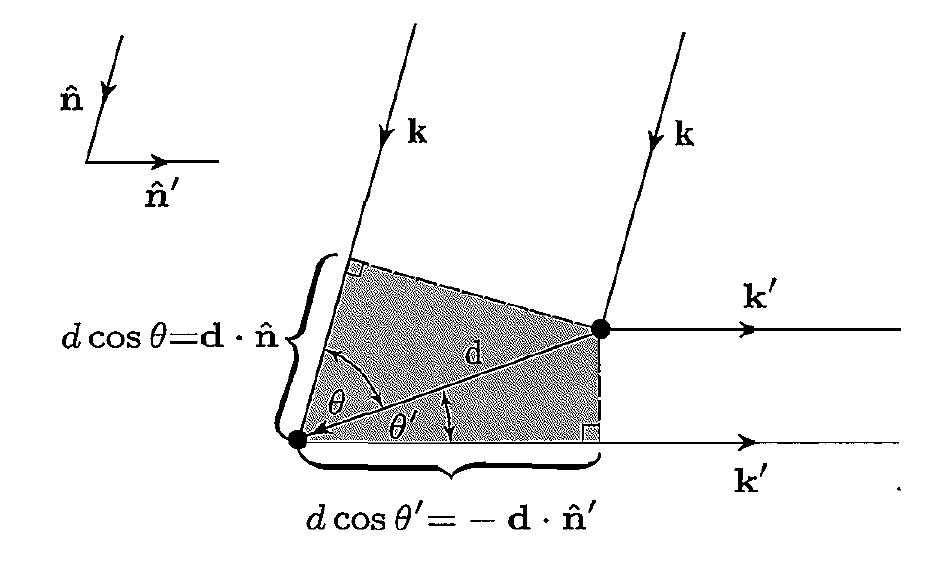
\includegraphics[width=0.5\textwidth]{../assets/theorie/lauebeugung}
    \caption{Skizze zur Erklärung der Laue-Bedingung. \imcitetwo[123]{Ashcroft}} \label{fig:laue}
\end{figure}
Zuerst betrachtet man die Bestrahlung zweier Gitterpunkte, deren Differenz durch den Vektor $\mathbf{O}$ gegeben ist,
mit Photonen unter Annahme elastischer Streuung.
Dabei ist die einfallende Strahlung durch den Wellenzahlvektor  $\mathbf{k}$ charakterisiert.
Es gilt die Dispersionsrelation $\lvert \mathbf{k} \rvert = 2 \pi / \lambda$.
Die gestreute Strahlung wird durch den Wellenvektor $\mathbf{k}'$ beschrieben.
Da nur elastische Streuung betrachtet wird, gilt $\lvert \mathbf{k} \rvert=\lvert \mathbf{k}' \rvert$.
Somit sind die Frequenzen ($\omega$ und $\omega'$) beider Wellen gleich.
Für den Wegunterschied findet man anhand \cref{fig:laue} den Zusammenhang:
\begin{equation*}
    \Delta s = \Delta s_{1} + \Delta s_{2} = \underbrace{ \mathbf{T} \cdot \frac{\mathbf{k}}{\lvert \mathbf{k} \rvert }
    -\mathbf{O}\cdot \frac{\mathbf{k}'}{\lvert \mathbf{k}' \rvert}  }_{ \text{Projektion von } \mathbf{O} \text{ auf }
    \mathbf{k} \text{ bzw. }\mathbf{k'} } =  \frac{\lambda}{2\pi} \mathbf{O}\cdot\Delta \mathbf{k}
\end{equation*}
Hierbei ist $\Delta \mathbf{k} = \mathbf{k}-\mathbf{k}'$.
Für konstruktive Interferenz ergibt sich die bekannte Bedingung $\Delta s = n \lambda$, sodass man durch Gleichsetzen
die Beziehung $\mathbf{O}\cdot\Delta \mathbf{k} =2\pi n$ erhält.
Aus der geometrischen Anordnungen der Gitterpunkte ergibt sich ein Wegunterschied, der äquivalent
zu einer Phasendifferenz von $\Delta\varphi=(2\pi / \lambda) \cdot \Delta s = \Delta \mathbf{k}\cdot \mathbf{O}$ ist.
\autocite[122-123]{Ashcroft}

\paragraph{Beschreibung durch Kugelwellen}
Betrachtet man nun die Überlagerung zweier Streuzentren, die durch den Vektor $\mathbf{O}$ voneinander verschoben sind,
so findet man folgenden Ausdruck:
\begin{align*}
    u(\mathbf{r},t)=u_{0}(\mathbf{r})\cdot \exp(\mathrm{i}\omega t+\mathrm{i}\lvert \mathbf{k}
    \rvert r) + u_{1}(\mathbf{r}) \cdot \exp(\mathrm{i}\omega t + \mathrm{i}\lvert \mathbf{k}
    \rvert r+\mathrm{i}\Delta\varphi)
\end{align*}
Die Überlagerung der beiden Wellen führt zu einer Interferenz, die durch die Phasendifferenz $\Delta\varphi$ bestimmt
wird.
Nun möchte man nicht über zwei Streuzentren, sondern über alle Gittervektoren im Kristall summieren.
Diese sind gegeben durch $\mathbf{O}_{pqr}=p\mathbf{a}_{1}+q\mathbf{a}_{2}+r\mathbf{a}_{3}$.
Dabei ändert Amplitude und Phase der einzelnen Kugelwellen, sodass man findet:
\begin{align*}
    u(\mathbf{r},t)
    &=\sum_{pqr} u_{pqr}(\mathbf{r})\cdot \exp(\mathrm{i}\omega t+\mathrm{i}
    \lvert \mathbf{k} \rvert r+\mathrm{i}\underbrace{ \Delta\varphi_{pqr} }_{ = \Delta
    \mathbf{k}\cdot \mathbf{O}_{pqr}})) \\
    &=\exp(\mathrm{i}\omega t+\mathrm{i}\lvert \mathbf{k} \rvert r)\cdot
    \underbrace{ \sum_{pqr}u_{pqr}(\mathbf{r})\cdot \exp(\mathrm{i}\Delta \mathbf{k}
    \cdot \mathbf{O}_{pqr}) }_{ \coloneqq A }
\end{align*}
Die Größe $A$ wird als Streuamplitude bezeichnet.
Die tatsächliche Streuung erfolgt an der Elektronenverteilung.
Das führt zu zusätzlichen Effekten wie den Atomformfaktor und den Strukturfaktor,
welche für weitere Betrachtungen jedoch vernachlässigt werden können.
\begin{equation*}
    A \propto \int n(\mathbf{r}) \exp(-\mathrm{i} \Delta \mathbf{k}\cdot
    \mathbf{r}) \, \mathrm{d}V(\mathbf{r})
\end{equation*}

\paragraph{Schlussfolgerung}
Damit die Streuamplitude maximal wird, muss die Interferenzbedingung $\mathbf{O}_{pqr}\cdot\Delta \mathbf{k} =2\pi n$
für alle $p$, $q$, $r$ gelten.
Zerlegt man $\mathbf{O}_{mnp}$ in seine Komponenten, erhält man folgende Gleichungen:
\begin{align*}
    \mathbf{a}_{1}\cdot\Delta \mathbf{k} &= 2\pi h \\
    \mathbf{a}_{2}\cdot\Delta \mathbf{k} &= 2\pi k \\
    \mathbf{a}_{3}\cdot\Delta \mathbf{k} &= 2\pi l \\
\end{align*}
Dies sind die Laue Gleichungen für Beugungsmaxima.
Sie sind erfüllt, falls $\Delta \mathbf{k}$ ein reziproker Gittervektor ist.
Für die Strukturamplitude ergibt sich anschließend:
\begin{equation*}
    A \propto \sum_{pqr} u_{pqr}(\mathbf{r}) \cdot\underbrace{ \exp(-\mathrm{i}
    \cdot2\pi\cdot(\underbrace{ mh+nk+pl }_{ \in\mathbb{Z} })) }_{ =1 }
\end{equation*}

\paragraph{Bragg-Bedingung}
Nun können wir mithilfe der Laue-Bedingung die Bragg-Bedingung herleiten.
Betrachtet man die einen Vektor $\Delta \mathbf{k}$, so ist sein Betrag gegeben durch:
\begin{align*}
    \lvert \Delta \mathbf{k} \rvert ^{2}&=\langle \Delta \mathbf{k} ,\Delta \mathbf{k}\rangle =\langle \mathbf{k}-\mathbf{k}', \mathbf{k}-\mathbf{k}' \rangle = k^{2}+k'^{2}-2kk'\cos(\alpha)  \\
    &=2{k}^{2}(1-\cos(\alpha))=4k^{2}\sin ^{2}\left( \frac{\alpha}{2} \right)
\end{align*}
Hierbei ist $\nu = \alpha / 2$ der Vragg
Da $\Delta \mathbf{k}$ ein Vektor aus dem reziproken Raum ist und senkrecht auf der Gitterebene
steht, an welcher er gestreut wird, existiert ein kürzester Vektor $\mathbf{g}$, sodass
$n\cdot \mathbf{g} =\Delta \mathbf{k}$.
Nach obiger Aussage wissen wir, dass $\mathbf{g}$ den Abstand der Netzebenen definiert
mit $d = 2 \pi \cdot\lvert \mathbf{g} \rvert ^{-1}$.
Daraus folgt $\lvert \Delta \mathbf{k} \rvert=n \lvert \mathbf{g} \rvert = 2\pi n/d$.
Kombiniert man beide Gleichungen miteinander, ergibt sich die Bragg-Bedingung:
\begin{align*}
    2k\sin(\nu)&=\frac{2\pi n}{d} \\
    2d\sin(\nu)&=n \lambda
\end{align*}
